\section{Introduction}

    \subparagraph{}Le but de ce {\color{info}6\ieme{} travail} est de réaliser une fonction logique à 3 entrées, 
    implémenter une porte logique CMOS et enfin de simuler le circuit avec le logiciel \textit{LTspice} afin de 
    démontrer l'exactitude des calculs.\\[1.5cm]
    
    \begin{titletbox}{À l'attention du correcteur / correctrice}{warning}
        N'hésitez pas à zoomer sur les schémas du circuit et autres images afin d'y voir plus clair.
    \end{titletbox}

    \section{Fonction logique}

    \subsection{Fonction pMOS}
    
        \subparagraph{}En pMOS, j'ai choisi la fonction suivante :
        
            \begin{equation*}
                \color{red}y\;=\;A \cdot \overline{B} + C
            \end{equation*}
            
    \subsection{Fonction nMOS}
    
    \subparagraph{}Pour trouver la fonction nMOS, il faut appliquer la formule de \textit{de Morgan} :
    
        {\color{green}\begin{align*}
            \overline{y}\;&=\;\overline{A \cdot \overline{B} + C} \\
            \overline{y}\;&=\;(\overline{A \cdot \overline{B}}) \cdot  \overline{C} \\
            \overline{y}\;&=\;(\overline{A} + {B}) \cdot  \overline{C} \\
            \overline{y}\;&=\;\overline{A} \cdot \overline{C} + B \cdot \overline{C} \\
            \overline{y}\;&=\;(\overline{A} + B) \cdot \overline{C}
        \end{align*}}
        
        \begin{empheq}[box=\fbox]{equation*}
        \color{red}
            \overline{y}\;=\;(\overline{A} + B) \cdot \overline{C}
        \end{empheq}
            
\section{Table de vérité}
    
    \subparagraph{}On trouve la table de vérité suivante :

    \begin{table}[H]
        \centering
        \begin{tabular}{c|c|c|c}
        A & B & C & {\color[HTML]{3166FF} Y} \\ \hline
        0 & 0 & 0 & {\color[HTML]{3166FF} 0} \\ \hline
        0 & 0 & 1 & {\color[HTML]{3166FF} 1} \\ \hline
        0 & 1 & 0 & {\color[HTML]{3166FF} 0} \\ \hline
        0 & 1 & 1 & {\color[HTML]{3166FF} 1} \\ \hline
        1 & 0 & 0 & {\color[HTML]{3166FF} 1} \\ \hline
        1 & 0 & 1 & {\color[HTML]{3166FF} 1} \\ \hline
        1 & 1 & 0 & {\color[HTML]{3166FF} 0} \\ \hline
        1 & 1 & 1 & {\color[HTML]{3166FF} 1}
        \end{tabular}
        \caption{Table de vérité de ma fonction logique}
        \label{table:ver}
    \end{table}
    
\section{Schéma du circuit CMOS}

    \subparagraph{}Pour dimensionner les transistors il y a des règles à respecter :
        \begin{enumerate}
            \item Longueur des transistors = $50n$
            \item Largeur d'un transistor nMOS : $10 \cdot longueur$
            \item Largeur d'un transistor pMOS : $20 \cdot longueur$
            \item Pour garder un rapport $\frac{w}{l}\;=\;1$, il faut diviser w par le nombre de transistor sur le chemin
        \end{enumerate}
        
    \subparagraph{}En appliquant ces règles, j'obtiens le circuit suivant :
        \begin{figure}[H]
            \centering
            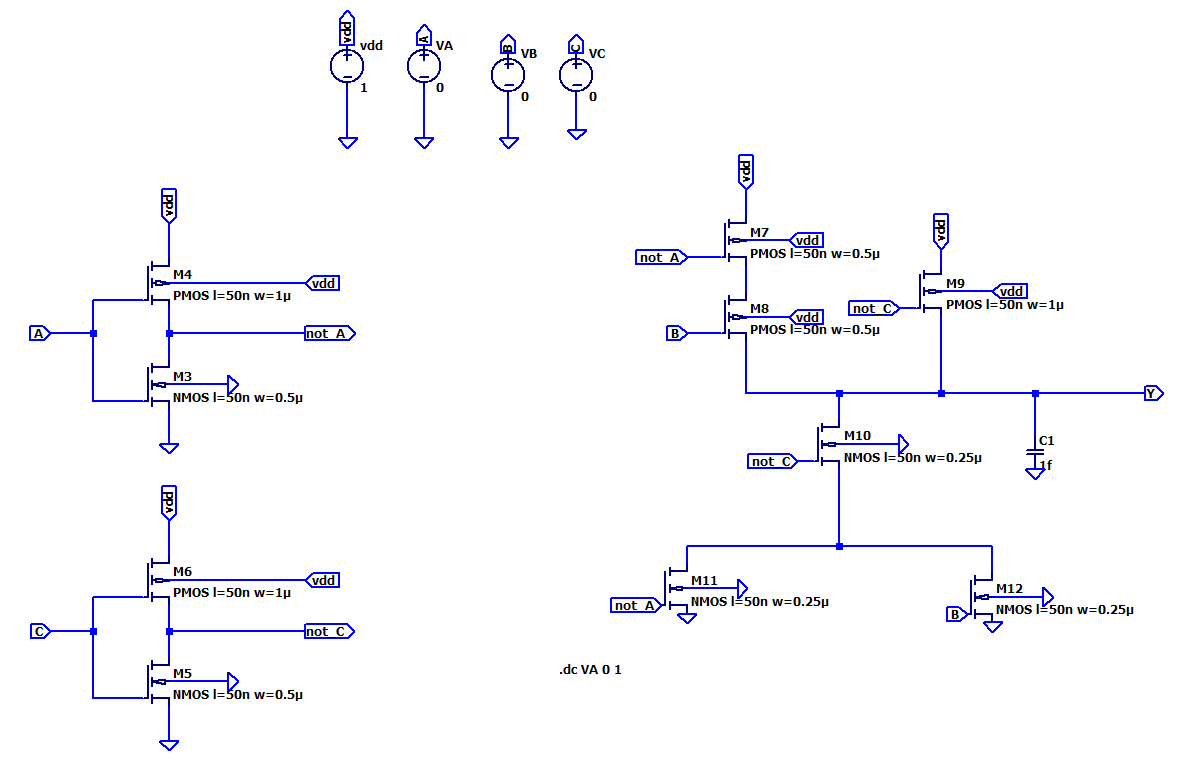
\includegraphics[scale=0.5]{../pictures/circuit.png}
            \caption{Schéma du circuit cMOS}
        \end{figure}
        
\section{Simulation .dc (variation d'une entrée)}

    \subparagraph{}Pour la simuation dc, je fais varier l'entrée A car (indépendamment de B et C) elle implique la relation Y = vdd.
    
        \begin{figure}[H]
            \centering
            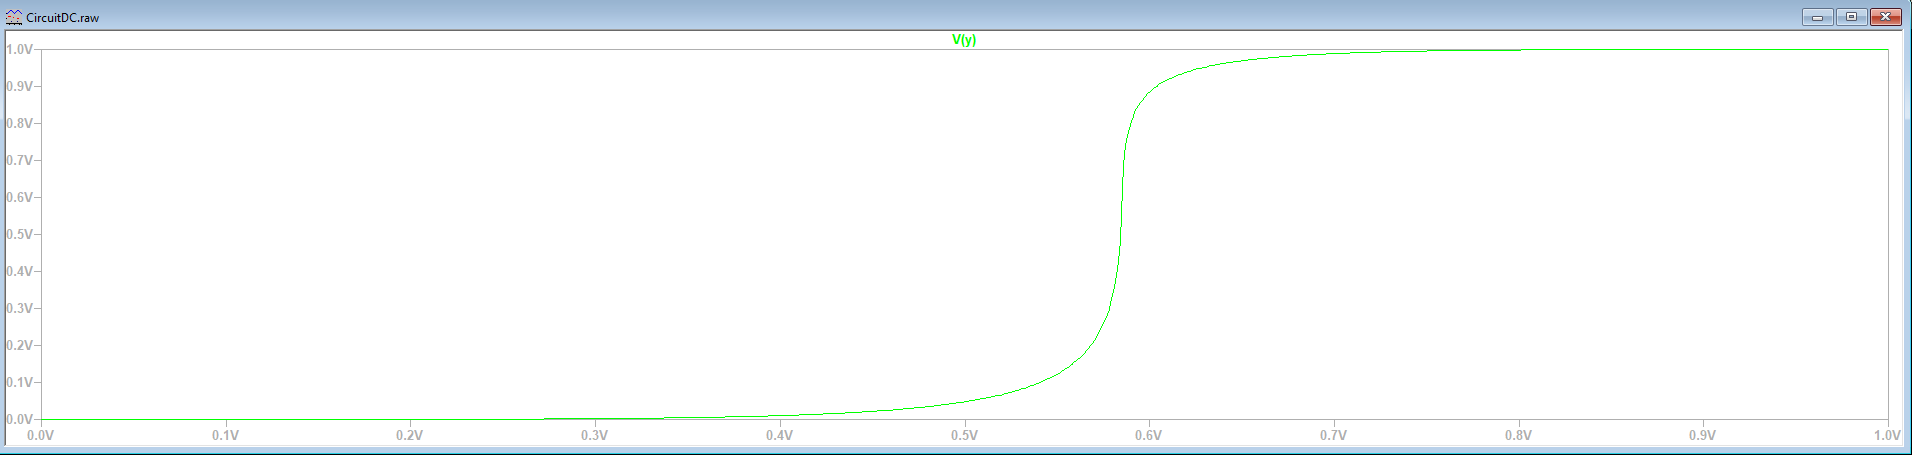
\includegraphics[scale=0.35]{../pictures/dc.png}
            \caption{Simulation en faisant varier A de 0 à 1 V}
        \end{figure}
\section{Simulation .tran (variation d'une entrée)}

    \subparagraph{}Pour cette simulation, je choisis de faire varier C, ainsi que de donner différentes valeurs pour la capacité (1f, 5f, 10f, 15f, 20f) et j'obtiens le circuit suivant :
    
        \begin{figure}[H]
            \centering
            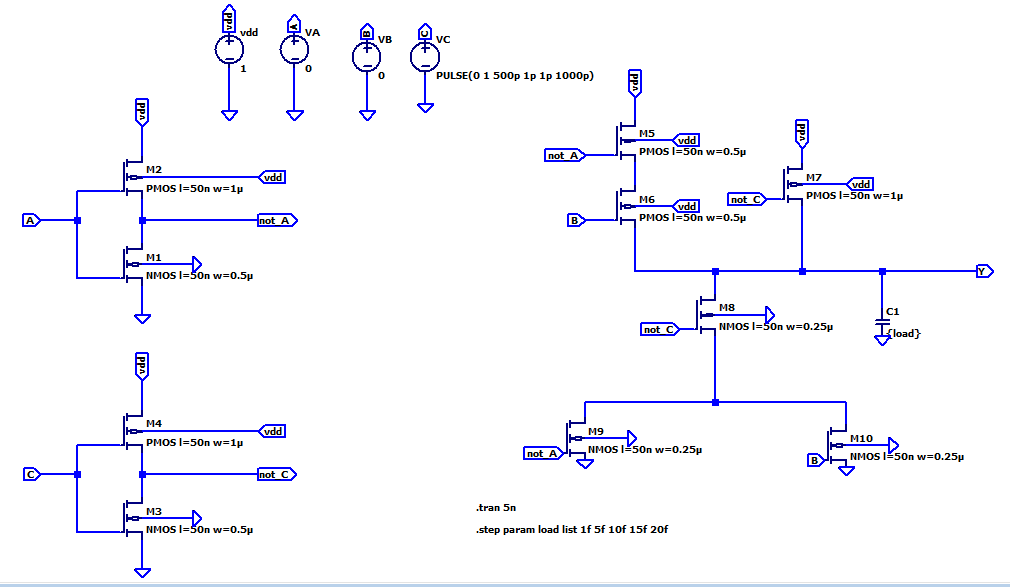
\includegraphics[scale=0.5]{../pictures/stepC.png}
            \caption{Schéma du circuit}
        \end{figure}
        

        \begin{figure}[H]
            \centering
            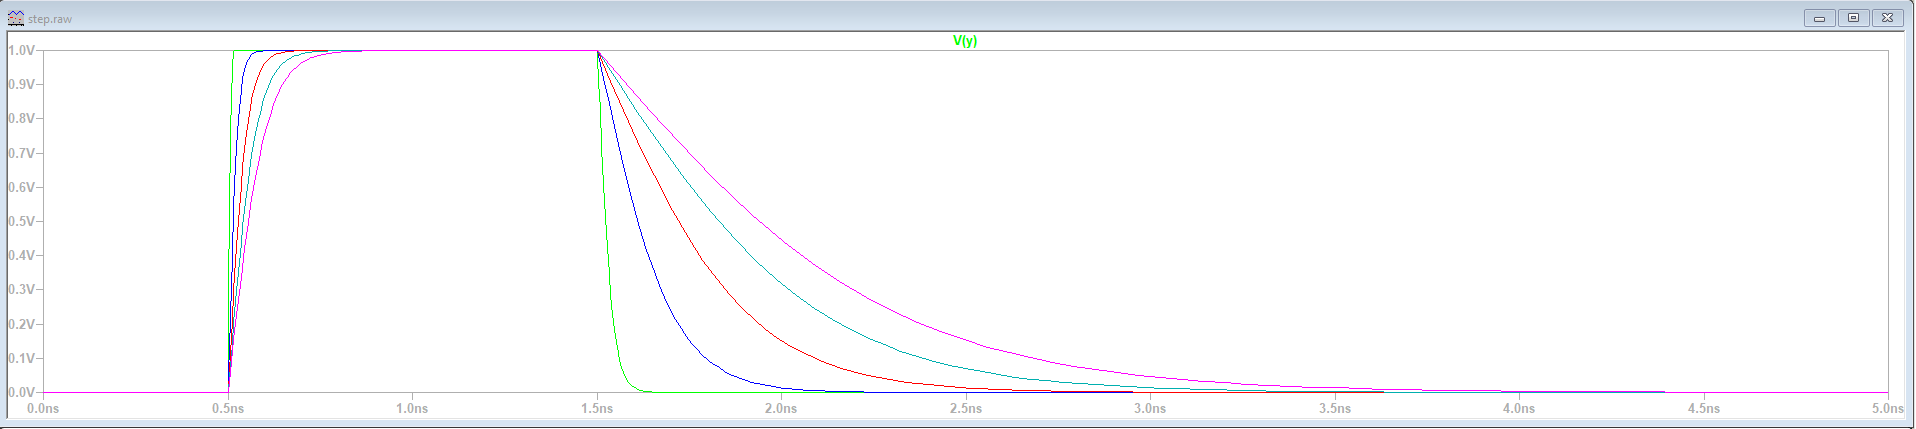
\includegraphics[scale=0.35]{../pictures/step.png}
            \caption{Simulation .tran en faisant varier une entrée}
        \end{figure}
        
\section{Simulation .tran (variation des 3 entrées)}

        \subparagraph{}Pour cette simulation, on fait varier toutes les entrées (voir les PULSE des sources) et obtient le circuit suivant : 

    
        \begin{figure}[H]
            \centering
            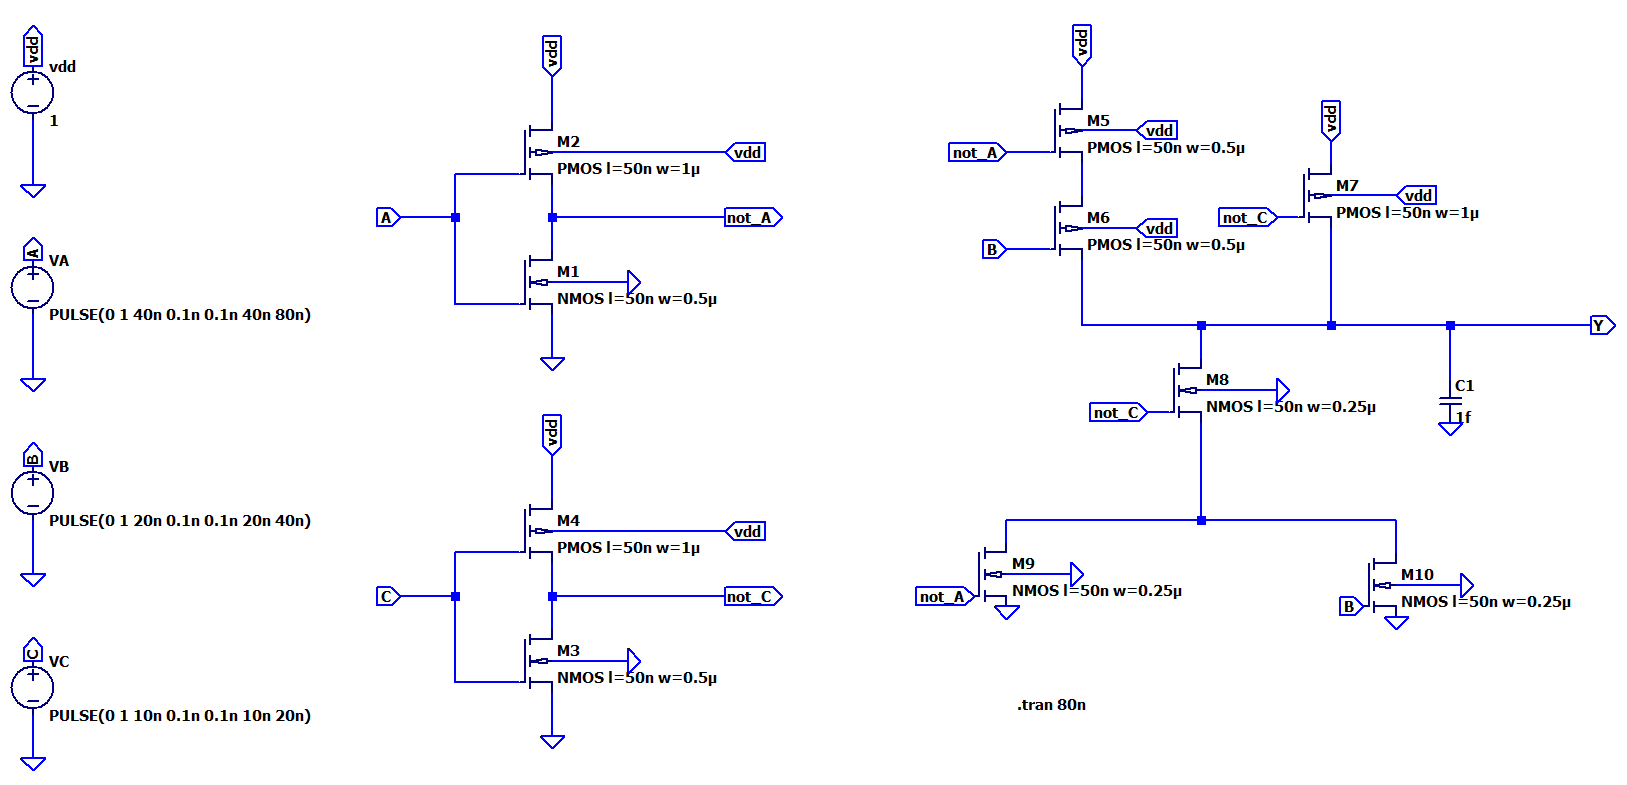
\includegraphics[scale=0.4]{../pictures/tranC.png}
            \caption{Schéma du circuit}
        \end{figure}

        \begin{figure}[H]
            \centering
            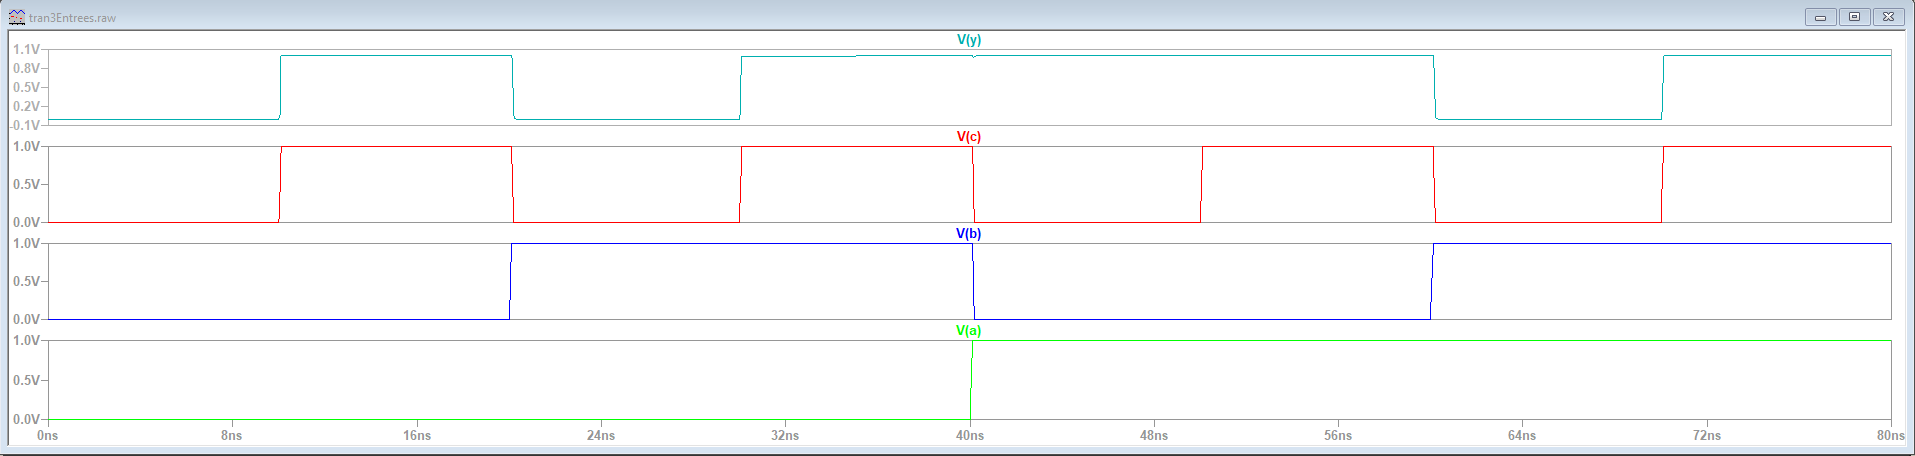
\includegraphics[scale=0.35]{../pictures/tran3.png}
            \caption{Simulation .tran en faisant varier les trois entrées}
        \end{figure}
        
\section{Conclusion}

    \subparagraph{}En premier lieu, on peut remarquer que la simulation en faisant varier les 3 entrées correspond bien à la table de vérité (voir \textbf{tableau \ref{table:ver}}) (les traits noirs symbolises la fin de la période) :
        
        \begin{figure}[H]
            \centering
            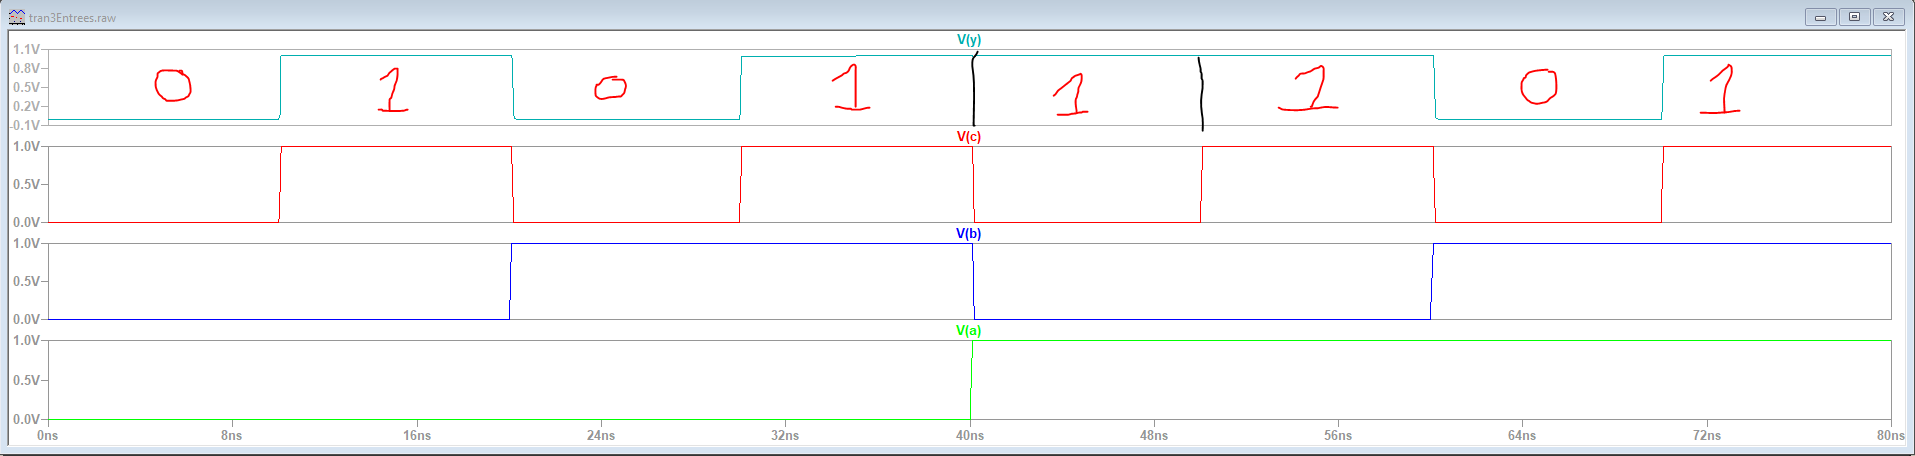
\includegraphics[scale=0.35]{../pictures/vérité.png}
            \caption{Lien avec la table de vérité}
        \end{figure}
        
    \subparagraph{}Pour conclure, j'ai correctement implémenter la fonction logique cMOS en y appliquant 
    beaucoup d'opérations pour ce travail et que les résultats fournis par \textit{LTspice} sont en accord avec 
    les résultats que j'ai trouvé. Ce travail est fort utile car il me permet de bien assimilé la logique des 
    transistors et par conséquent de mieux comprendre le fonctionnement d'un ordinateur.

\end{document}